% Options for packages loaded elsewhere
\PassOptionsToPackage{unicode}{hyperref}
\PassOptionsToPackage{hyphens}{url}
%
\documentclass[
  man,floatsintext]{apa6}
\usepackage{amsmath,amssymb}
\usepackage{lmodern}
\usepackage{iftex}
\ifPDFTeX
  \usepackage[T1]{fontenc}
  \usepackage[utf8]{inputenc}
  \usepackage{textcomp} % provide euro and other symbols
\else % if luatex or xetex
  \usepackage{unicode-math}
  \defaultfontfeatures{Scale=MatchLowercase}
  \defaultfontfeatures[\rmfamily]{Ligatures=TeX,Scale=1}
\fi
% Use upquote if available, for straight quotes in verbatim environments
\IfFileExists{upquote.sty}{\usepackage{upquote}}{}
\IfFileExists{microtype.sty}{% use microtype if available
  \usepackage[]{microtype}
  \UseMicrotypeSet[protrusion]{basicmath} % disable protrusion for tt fonts
}{}
\makeatletter
\@ifundefined{KOMAClassName}{% if non-KOMA class
  \IfFileExists{parskip.sty}{%
    \usepackage{parskip}
  }{% else
    \setlength{\parindent}{0pt}
    \setlength{\parskip}{6pt plus 2pt minus 1pt}}
}{% if KOMA class
  \KOMAoptions{parskip=half}}
\makeatother
\usepackage{xcolor}
\usepackage{graphicx}
\makeatletter
\def\maxwidth{\ifdim\Gin@nat@width>\linewidth\linewidth\else\Gin@nat@width\fi}
\def\maxheight{\ifdim\Gin@nat@height>\textheight\textheight\else\Gin@nat@height\fi}
\makeatother
% Scale images if necessary, so that they will not overflow the page
% margins by default, and it is still possible to overwrite the defaults
% using explicit options in \includegraphics[width, height, ...]{}
\setkeys{Gin}{width=\maxwidth,height=\maxheight,keepaspectratio}
% Set default figure placement to htbp
\makeatletter
\def\fps@figure{htbp}
\makeatother
\setlength{\emergencystretch}{3em} % prevent overfull lines
\providecommand{\tightlist}{%
  \setlength{\itemsep}{0pt}\setlength{\parskip}{0pt}}
\setcounter{secnumdepth}{-\maxdimen} % remove section numbering
% Make \paragraph and \subparagraph free-standing
\ifx\paragraph\undefined\else
  \let\oldparagraph\paragraph
  \renewcommand{\paragraph}[1]{\oldparagraph{#1}\mbox{}}
\fi
\ifx\subparagraph\undefined\else
  \let\oldsubparagraph\subparagraph
  \renewcommand{\subparagraph}[1]{\oldsubparagraph{#1}\mbox{}}
\fi
\newlength{\cslhangindent}
\setlength{\cslhangindent}{1.5em}
\newlength{\csllabelwidth}
\setlength{\csllabelwidth}{3em}
\newlength{\cslentryspacingunit} % times entry-spacing
\setlength{\cslentryspacingunit}{\parskip}
\newenvironment{CSLReferences}[2] % #1 hanging-ident, #2 entry spacing
 {% don't indent paragraphs
  \setlength{\parindent}{0pt}
  % turn on hanging indent if param 1 is 1
  \ifodd #1
  \let\oldpar\par
  \def\par{\hangindent=\cslhangindent\oldpar}
  \fi
  % set entry spacing
  \setlength{\parskip}{#2\cslentryspacingunit}
 }%
 {}
\usepackage{calc}
\newcommand{\CSLBlock}[1]{#1\hfill\break}
\newcommand{\CSLLeftMargin}[1]{\parbox[t]{\csllabelwidth}{#1}}
\newcommand{\CSLRightInline}[1]{\parbox[t]{\linewidth - \csllabelwidth}{#1}\break}
\newcommand{\CSLIndent}[1]{\hspace{\cslhangindent}#1}
\ifLuaTeX
\usepackage[bidi=basic]{babel}
\else
\usepackage[bidi=default]{babel}
\fi
\babelprovide[main,import]{english}
% get rid of language-specific shorthands (see #6817):
\let\LanguageShortHands\languageshorthands
\def\languageshorthands#1{}
% Manuscript styling
\usepackage{upgreek}
\captionsetup{font=singlespacing,justification=justified}

% Table formatting
\usepackage{longtable}
\usepackage{lscape}
% \usepackage[counterclockwise]{rotating}   % Landscape page setup for large tables
\usepackage{multirow}		% Table styling
\usepackage{tabularx}		% Control Column width
\usepackage[flushleft]{threeparttable}	% Allows for three part tables with a specified notes section
\usepackage{threeparttablex}            % Lets threeparttable work with longtable

% Create new environments so endfloat can handle them
% \newenvironment{ltable}
%   {\begin{landscape}\centering\begin{threeparttable}}
%   {\end{threeparttable}\end{landscape}}
\newenvironment{lltable}{\begin{landscape}\centering\begin{ThreePartTable}}{\end{ThreePartTable}\end{landscape}}

% Enables adjusting longtable caption width to table width
% Solution found at http://golatex.de/longtable-mit-caption-so-breit-wie-die-tabelle-t15767.html
\makeatletter
\newcommand\LastLTentrywidth{1em}
\newlength\longtablewidth
\setlength{\longtablewidth}{1in}
\newcommand{\getlongtablewidth}{\begingroup \ifcsname LT@\roman{LT@tables}\endcsname \global\longtablewidth=0pt \renewcommand{\LT@entry}[2]{\global\advance\longtablewidth by ##2\relax\gdef\LastLTentrywidth{##2}}\@nameuse{LT@\roman{LT@tables}} \fi \endgroup}

% \setlength{\parindent}{0.5in}
% \setlength{\parskip}{0pt plus 0pt minus 0pt}

% Overwrite redefinition of paragraph and subparagraph by the default LaTeX template
% See https://github.com/crsh/papaja/issues/292
\makeatletter
\renewcommand{\paragraph}{\@startsection{paragraph}{4}{\parindent}%
  {0\baselineskip \@plus 0.2ex \@minus 0.2ex}%
  {-1em}%
  {\normalfont\normalsize\bfseries\itshape\typesectitle}}

\renewcommand{\subparagraph}[1]{\@startsection{subparagraph}{5}{1em}%
  {0\baselineskip \@plus 0.2ex \@minus 0.2ex}%
  {-\z@\relax}%
  {\normalfont\normalsize\itshape\hspace{\parindent}{#1}\textit{\addperi}}{\relax}}
\makeatother

% \usepackage{etoolbox}
\makeatletter
\patchcmd{\HyOrg@maketitle}
  {\section{\normalfont\normalsize\abstractname}}
  {\section*{\normalfont\normalsize\abstractname}}
  {}{\typeout{Failed to patch abstract.}}
\patchcmd{\HyOrg@maketitle}
  {\section{\protect\normalfont{\@title}}}
  {\section*{\protect\normalfont{\@title}}}
  {}{\typeout{Failed to patch title.}}
\makeatother

\usepackage{xpatch}
\makeatletter
\xapptocmd\appendix
  {\xapptocmd\section
    {\addcontentsline{toc}{section}{\appendixname\ifoneappendix\else~\theappendix\fi\\: #1}}
    {}{\InnerPatchFailed}%
  }
{}{\PatchFailed}
\keywords{keywords\newline\indent Word count: X}
\usepackage{lineno}

\linenumbers
\usepackage{csquotes}
\ifLuaTeX
  \usepackage{selnolig}  % disable illegal ligatures
\fi
\IfFileExists{bookmark.sty}{\usepackage{bookmark}}{\usepackage{hyperref}}
\IfFileExists{xurl.sty}{\usepackage{xurl}}{} % add URL line breaks if available
\urlstyle{same} % disable monospaced font for URLs
\hypersetup{
  pdftitle={A survey of registration practices among observational researchers using preexisting datasets},
  pdfauthor={Robert T. Thibault1,5, Marton Kovacs2,6, Tom E. Hardwicke3, Alexandra Sarafoglou4, John P. A. Ioannidis4, \& Marcus R. Munafò1,7},
  pdflang={en-EN},
  pdfkeywords={keywords},
  hidelinks,
  pdfcreator={LaTeX via pandoc}}

\title{A survey of registration practices among observational researchers using preexisting datasets}
\author{Robert T. Thibault\textsuperscript{1,5}, Marton Kovacs\textsuperscript{2,6}, Tom E. Hardwicke\textsuperscript{3}, Alexandra Sarafoglou\textsuperscript{4}, John P. A. Ioannidis\textsuperscript{4}, \& Marcus R. Munafò\textsuperscript{1,7}}
\date{}


\shorttitle{Explore and Confirm Analysis Workflow}

\authornote{

The authors made the following contributions. Robert T. Thibault: Conceptualization, Data curation, Formal analysis, Funding acquisition, Investigation, Methodology, Project administration, Resources, Supervision, Validation, Visualization, Writing - original draft, Writing - review \& editing; Marton Kovacs: Data curation, Formal analysis, Software, Validation, Visualization, Writing - review \& editing; Tom E. Hardwicke: Methodology, Writing - review \& editing; Alexandra Sarafoglou: Methodology, Writing - review \& editing; John P. A. Ioannidis: Methodology, Writing - review \& editing; Marcus R. Munafò: Conceptualization, Methodology, Supervision, Writing - review \& editing.

Correspondence concerning this article should be addressed to Robert T. Thibault, Enter postal address here. E-mail: \href{mailto:robert.thibault@stanford.edu}{\nolinkurl{robert.thibault@stanford.edu}}

}

\affiliation{\vspace{0.5cm}\textsuperscript{1} Meta-Research Innovation Center at Stanford (METRICS), Stanford University.\\\textsuperscript{2} Doctoral School of Psychology, ELTE Eotvos Lorand University, Budapest, Hungary\\\textsuperscript{3} Melbourne School of Psychological Sciences, University of Melbourne.\\\textsuperscript{4} Department of Psychology, University of Amsterdam.\\\textsuperscript{5} School of Psychological Science, University of Bristol.\\\textsuperscript{6} Institute of Psychology, ELTE Eotvos Lorand University, Budapest, Hungary\\\textsuperscript{7} Meta-Research Innovation Center Berlin (METRIC-B), QUEST Center for Transforming Biomedical Research, Berlin Institute of Health, Charité -- Universitätsmedizin Berlin.\\\textsuperscript{8} MRC Integrative Epidemiology Unit at the University of Bristol.\\\textsuperscript{9} Departments of Medicine, Epidemiology and Population Health, Biomedical Data Science, and Statistics, Stanford University.}

\abstract{%
placeholder for an abstract
}



\begin{document}
\maketitle

\hypertarget{introduction}{%
\section{Introduction}\label{introduction}}

\hypertarget{methods}{%
\section{Methods}\label{methods}}

\hypertarget{results}{%
\section{Results}\label{results}}

\hypertarget{participants}{%
\subsection{Participants}\label{participants}}

We invited the ALSPAC mailing list to participate, which included 1148 email addresses. 54 emails bounced, leaving 1094 emails that went through. The survey was completed 107 times and partially completed 21 times, leading to a response rate of 10\% for complete surveys and 2\% for incomplete surveys.\footnote{The ALSPAC mailing list has been active for \textgreater30 years and may contain email addresses that are no longer monitored. For example, we received one email reply stating that the recipient hasn't been active in research for 30 years. Excluding these email addresses would increase the response rate, but we do not know by how much.} The median time taken for complete survey responses was 7.22 minutes (IQR: 4.30 to 13.10).

Respondents published a median of NA (IQR 2 to 25) studies using preexisting observational data (Figure S1). They reported using the programming languages R (n = 65), Stata (n = 48), SPSS (n = 17), SAS (n = 15), Python (n = 6), Mplus (n = 3), Bash (n = 2), MATLAB (n = 1), Nextflow (n = 1), and plink2 (n = 1) (Table S1)\footnote{Participants could select multiple responses to this survey question.}. 61\% of participants reported being more concerned with research trustworthiness, bias, rigour, and reproducibility compared to what they think of as a typical research who uses preexisting observational data (Figure C2); 6\% reported being less concerned.

\hypertarget{survey-results}{%
\subsection{Survey results}\label{survey-results}}

\begin{figure}

{\centering 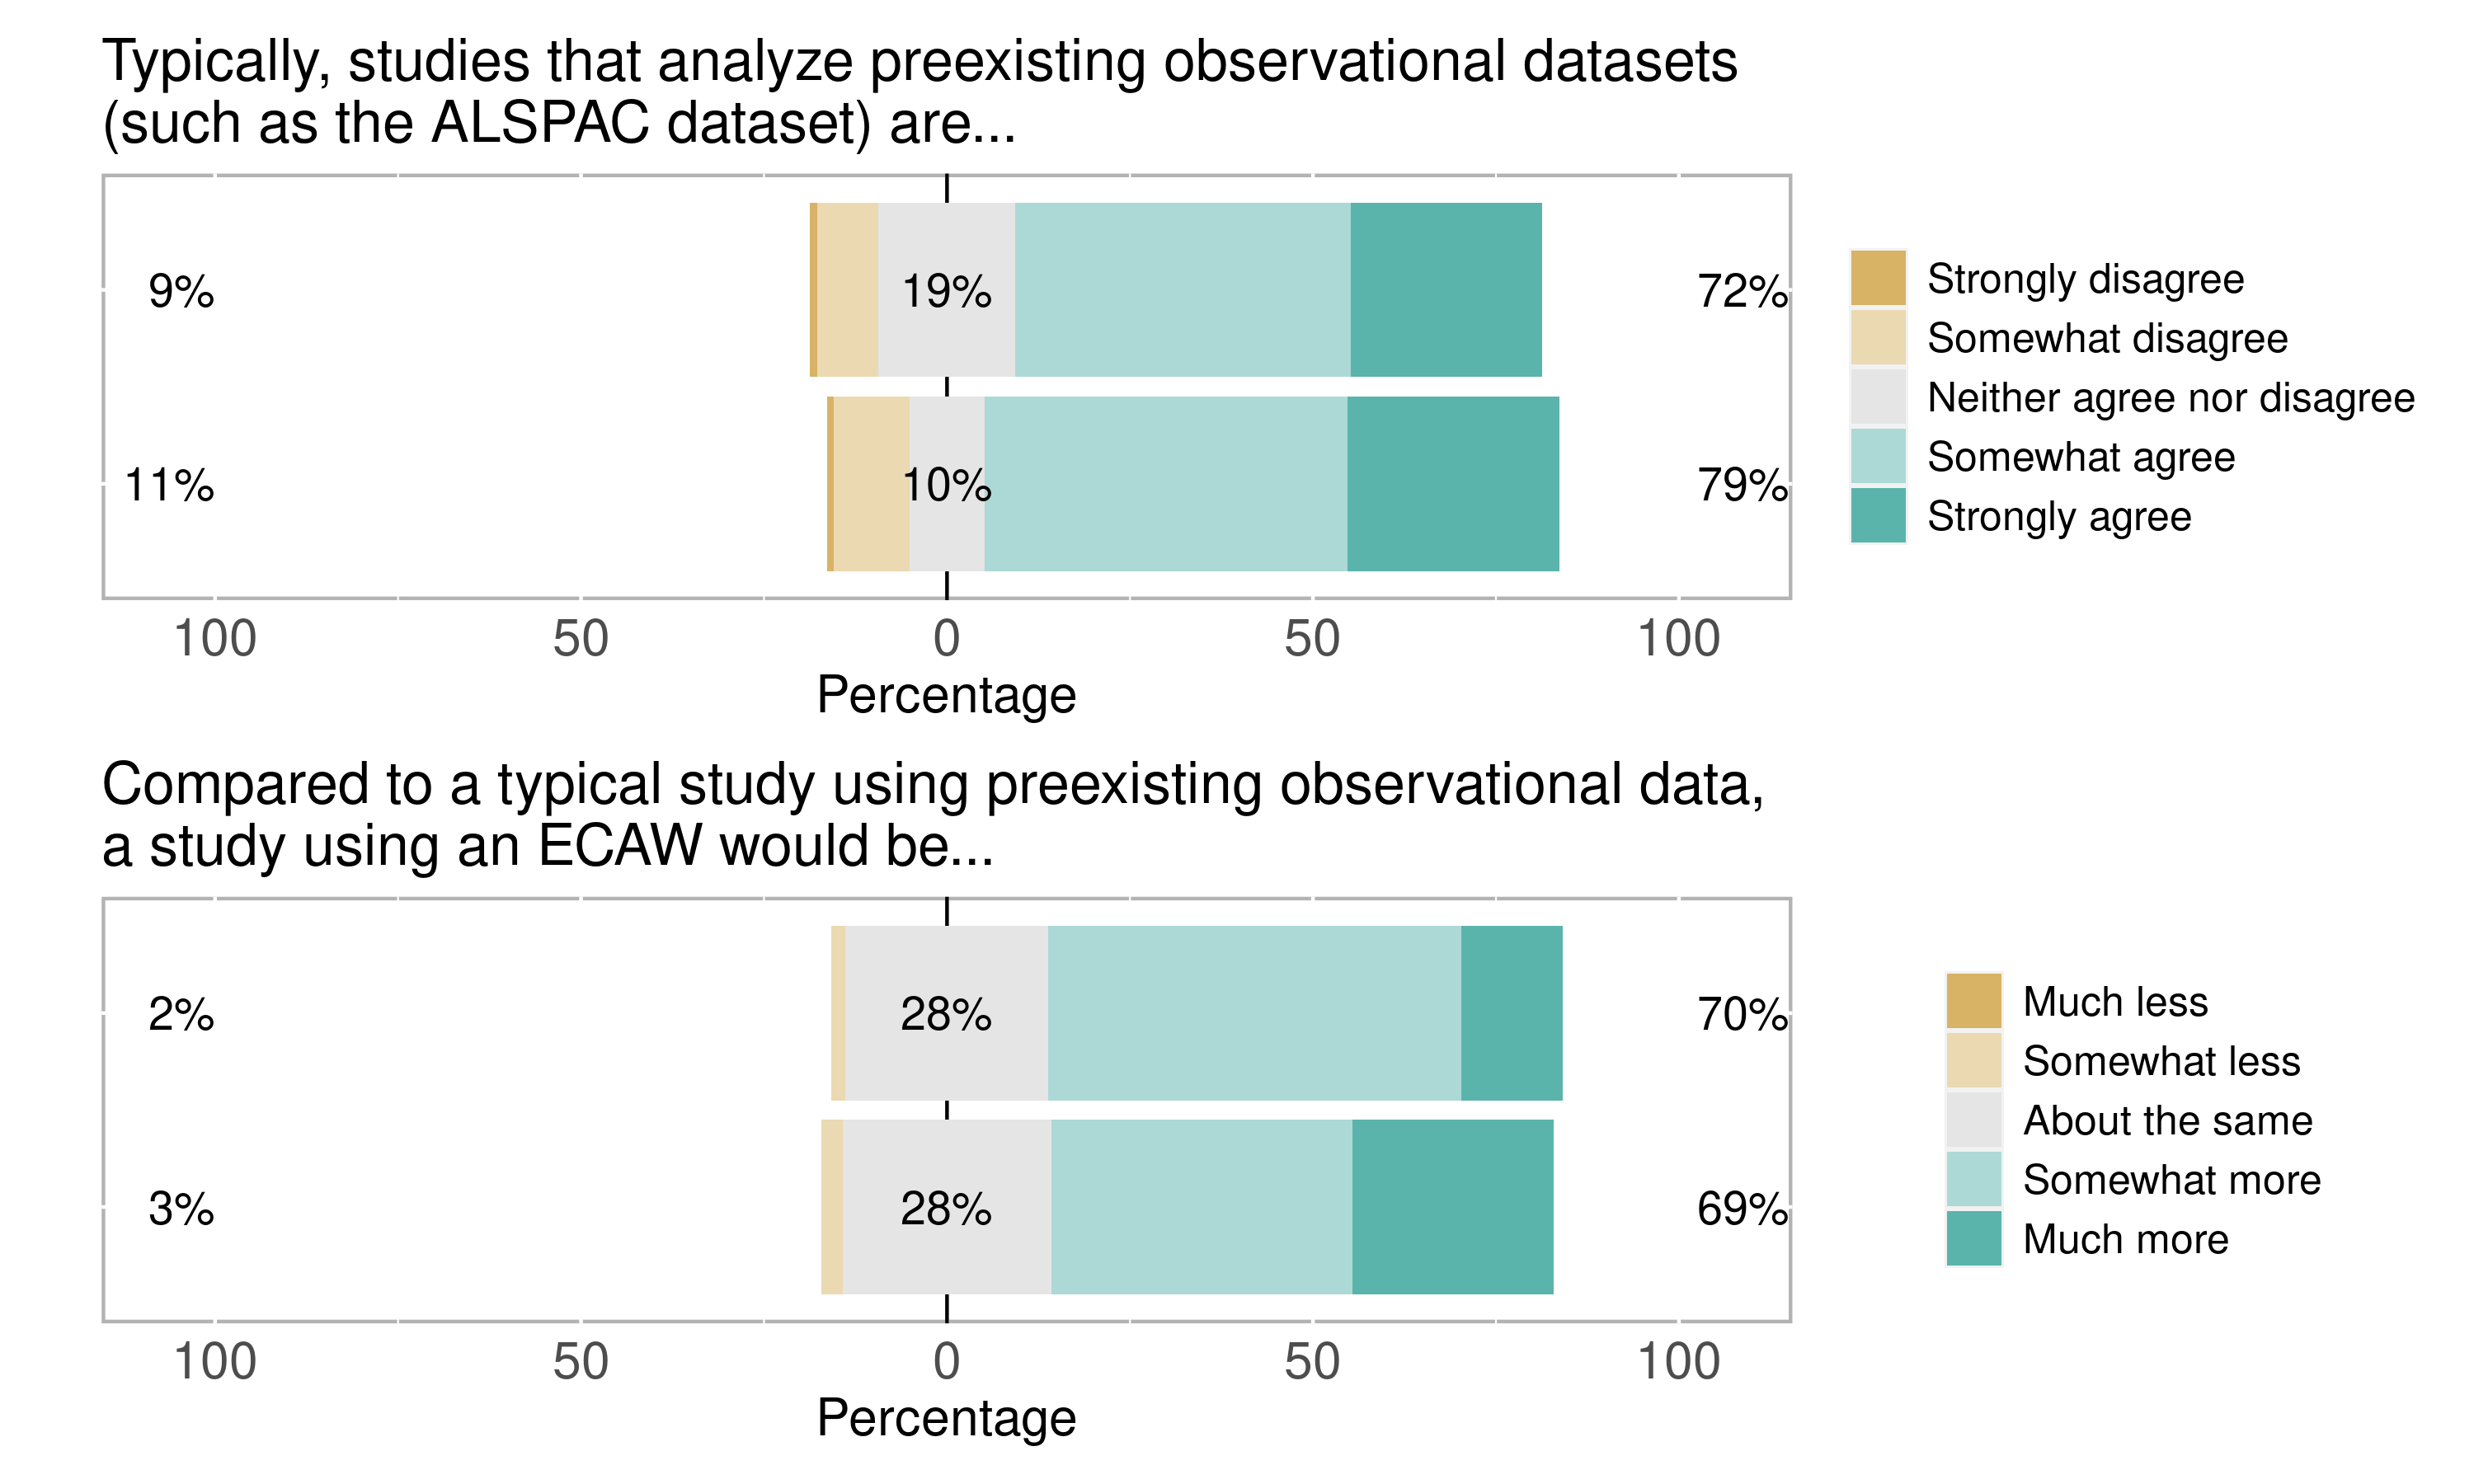
\includegraphics[width=1\linewidth]{manuscript_files/figure-latex/typicallyEcawPlot-1} 

}

\caption{Caption goes here...}\label{fig:typicallyEcawPlot}
\end{figure}

Respondents generally agreed that studies that analyze preexisting observational datasets are trustworthy\footnote{The survey defined trustworthy as: ``meaning that the results and conclusions of the publications are valid, reliable, rigorous, and accurate. That they merit trust.''} (72\%) and reproducible\footnote{The survey defined reproducible ``in the sense that other researchers re-analysing the data with the same research question would produce similar results.''} (79\%) (Figure 1A). At the same time, many agreed that a study using an ECAW would be \emph{more} trustworthy (70\%) and \emph{more} reproducible (69\%) compared to a typical study using preexisting observational data (Figure 1B).

Over half of respondents reported that their studies using preexisting observational data are preregistered never or almost never (38\%), or sometimes (27\%) (Figure 2A). About half reported sharing their analysis scripts never or almost never (20\%), or sometimes (32\%) (Figure 2B). 79\% reported that they never or almost never blind the data analyst (Figure 2C). Almost all respondents answered that they use both exploratory (95\%) and confirmatory (92\%) analyses at least sometimes (Figure 2D-E).

\begin{figure}

{\centering 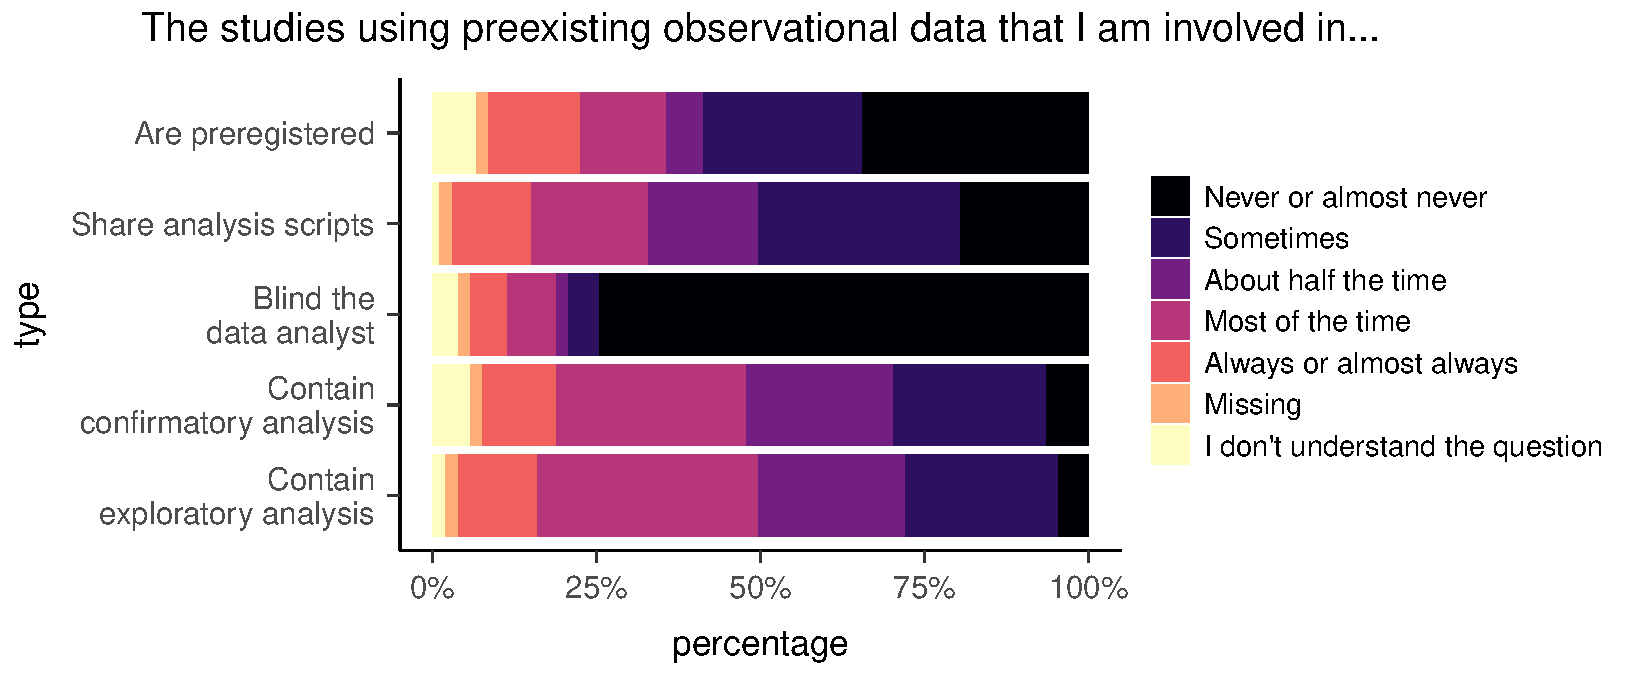
\includegraphics[width=1\linewidth]{manuscript_files/figure-latex/methodPlot-1} 

}

\caption{Caption goes here...}\label{fig:methodPlot}
\end{figure}

25\% of respondents agreed (versus 44\% who disagreed) that they would be less willing to use ALSPAC data if they were required to use an ECAW (Figure 3). 53\% agreed (20\% disagreed) that they would opt-in if ALSPAC ran a study on ECAWs. 55\% agreed (10\% disagreed) that ALSPAC should run a study on ECAWs. 45\% agreed (22\% disagreed) that they would prefer using an ECAW than using typical preregistration.

\begin{figure}

{\centering 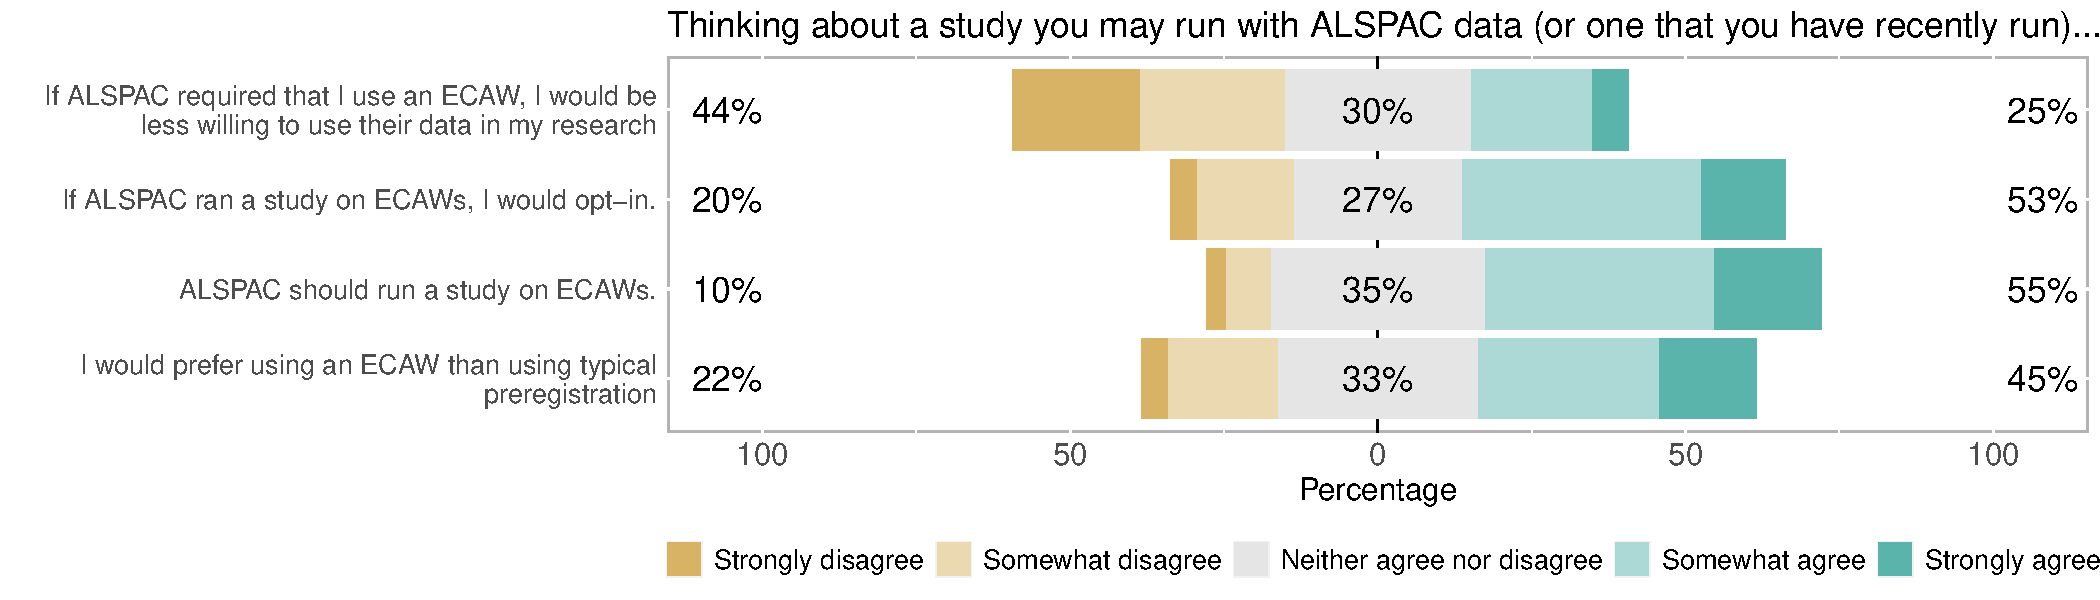
\includegraphics[width=1\linewidth]{manuscript_files/figure-latex/alspacPlot-1} 

}

\caption{Caption goes here...}\label{fig:alspacPlot}
\end{figure}

Table 1. Recurring topics in responses to the open-ended survey questions. The survey included 4 open-ended questions with broad prompts regarding running a study on ECAWs, benefits and drawbacks of ECAWs, related research practices, and general comments. These questions received a total of (92) responses from (55) unique respondents. A complete list of responses are viewable in the open data {[}LINK{]}. We synthesized the response to open-ended questions into the 9 topics on the left side of this table. We divide these into three sections: (i) concerns about the acceptability of ECAWs, (ii) concerns that ECAWs will not have their intended impact, and (iii) alternative interventions that may achieve similar goals as typical preregistration and ECAWs. On the right side of the table, we provide a reflection on each topic.

\hypertarget{exploratory-analyses}{%
\subsection{Exploratory analyses}\label{exploratory-analyses}}

\hypertarget{discussion}{%
\section{Discussion}\label{discussion}}

\hypertarget{acknowledgements}{%
\section{Acknowledgements}\label{acknowledgements}}

\newpage

\hypertarget{references}{%
\section{References}\label{references}}

\hypertarget{refs}{}
\begin{CSLReferences}{0}{0}
\end{CSLReferences}


\end{document}
